\documentclass{beamer}
\usepackage[utf8]{inputenc}
\usepackage{polski}
\usepackage[polish]{babel}
\usepackage[T1]{fontenc}
\usepackage{multicol}
\usepackage{amsmath}
\usepackage{mathtools}

\mode<presentation>
{
  \usetheme{Madrid}
  \usecolortheme{beaver}
  \usefonttheme{default}
  \setbeamertemplate{navigation symbols}{}
  \setbeamertemplate{caption}[numbered]
} 


\usepackage{graphicx}
\DeclareGraphicsExtensions{.png,.jpg}

\title[Elasticsearch]{Elasticsearch}
\author{Jakub Podeszwik}
\institute{Yameo}
\date{28.03.2019}

\AtBeginSection[]{
	\begin{frame}
		\begin{center}
			\usebeamerfont{section title}\Large\insertsection
		\end{center}
	\end{frame}
}

\begin{document}

\begin{frame}
  \titlepage
\end{frame}

\begin{frame}{Inverted index}
	\begin{figure}
		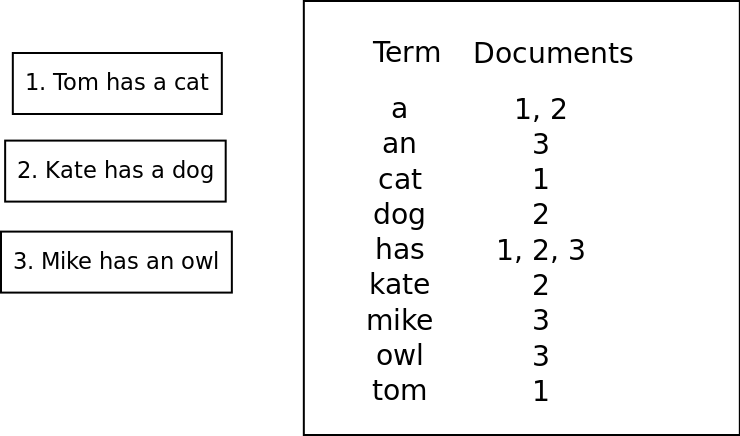
\includegraphics[width=\textwidth,height=7cm,keepaspectratio=true]{inverted-index}
	\end{figure}
\end{frame}

\begin{frame}{Lucene index}
	\begin{figure}
		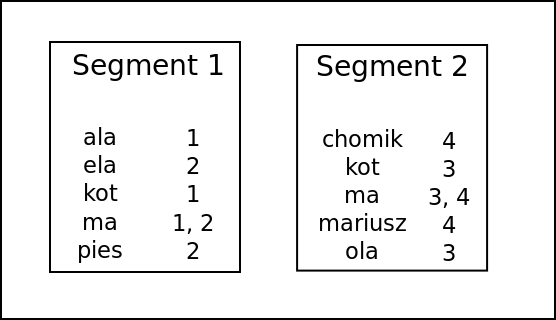
\includegraphics[width=\textwidth,height=7cm,keepaspectratio=true]{lucene-index}
	\end{figure}
\end{frame}
\begin{frame}{Elasticsearch index}
	\begin{figure}
		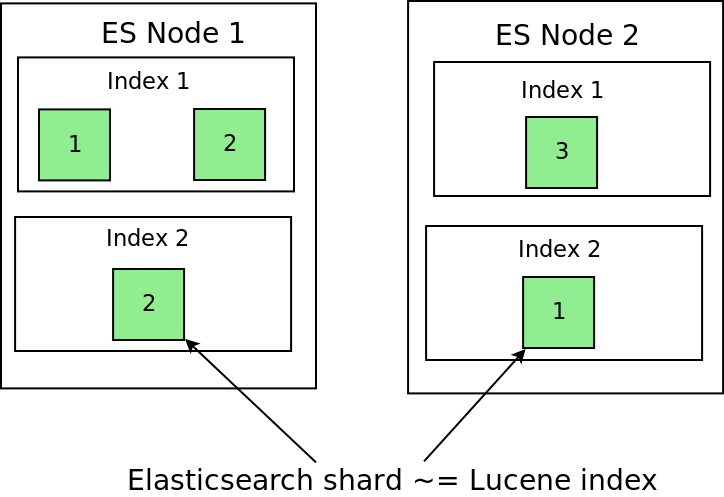
\includegraphics[width=\textwidth,height=7cm,keepaspectratio=true]{elasticsearch-index}
	\end{figure}
\end{frame}
\begin{frame}{Translog}
	\begin{figure}
		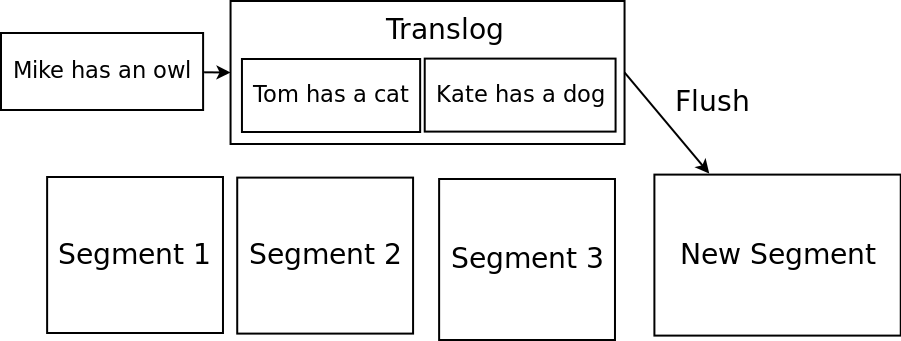
\includegraphics[width=\textwidth,height=7cm,keepaspectratio=true]{translog}
	\end{figure}
\end{frame}
\begin{frame}{Search}
	\begin{figure}
		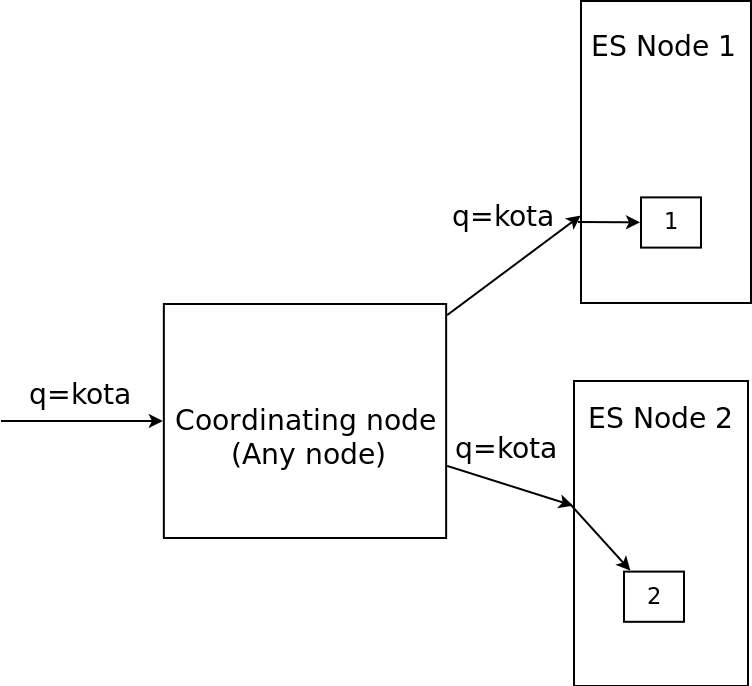
\includegraphics[width=\textwidth,height=7cm,keepaspectratio=true]{search1}
	\end{figure}
\end{frame}
\begin{frame}{Search}
	\begin{figure}
		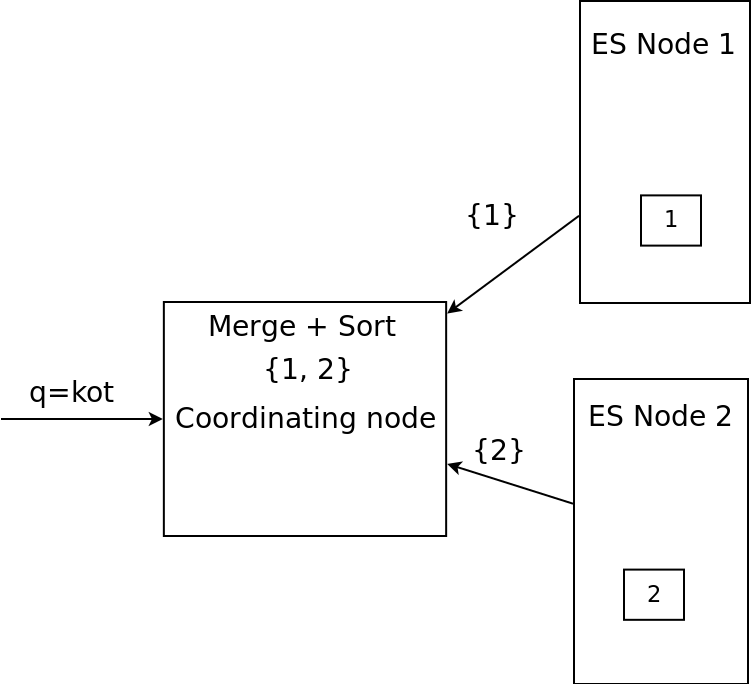
\includegraphics[width=\textwidth,height=7cm,keepaspectratio=true]{search2}
	\end{figure}
\end{frame}
\begin{frame}{Search}
	\begin{figure}
		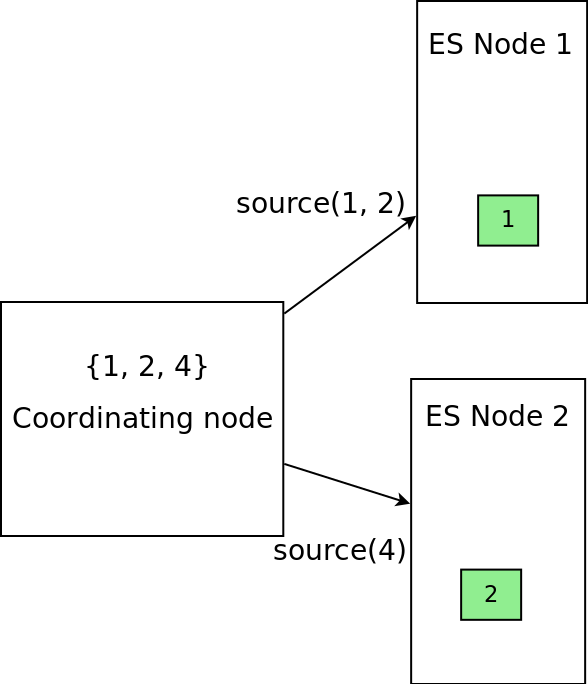
\includegraphics[width=\textwidth,height=7cm,keepaspectratio=true]{search3}
	\end{figure}
\end{frame}
\begin{frame}{Search}
	\begin{figure}
		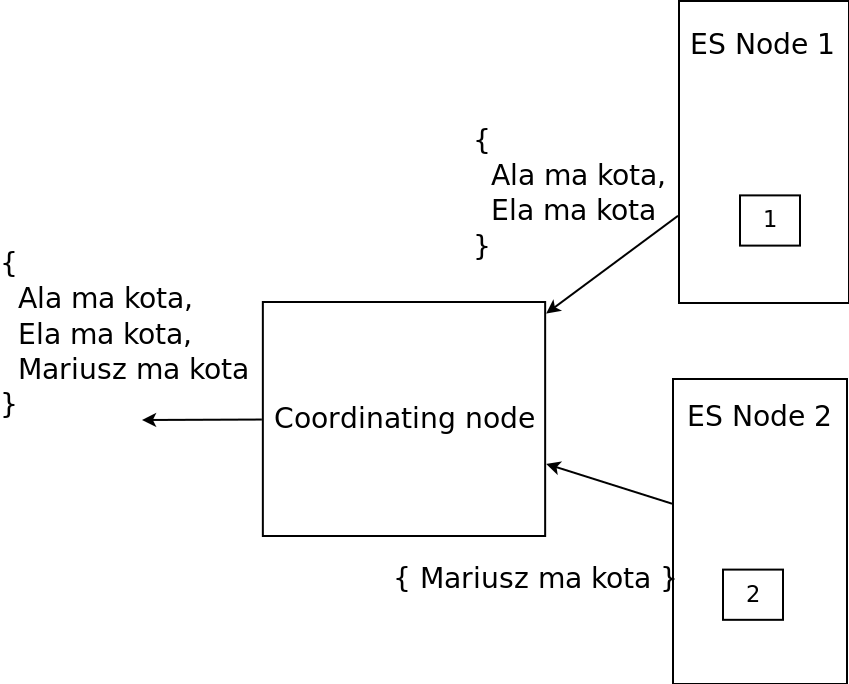
\includegraphics[width=\textwidth,height=7cm,keepaspectratio=true]{search4}
	\end{figure}
\end{frame}
\begin{frame}{Indexing}
	\begin{figure}
		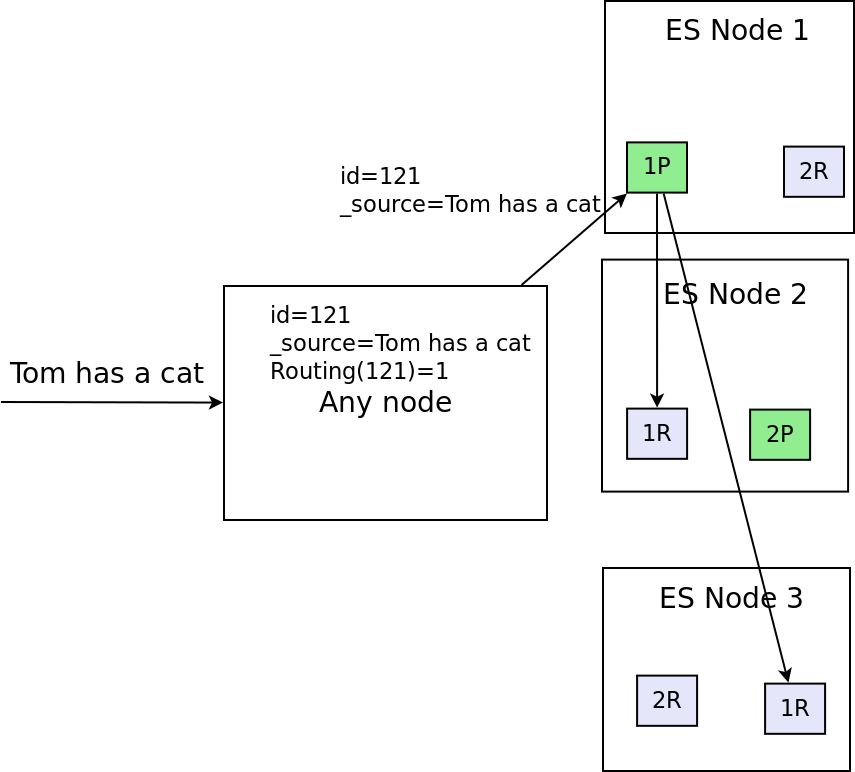
\includegraphics[width=\textwidth,height=7cm,keepaspectratio=true]{indexing}
	\end{figure}
\end{frame}
\begin{frame}{Scoring}
	\begin{equation*}
	\begin{multlined}
score(q,d) = \\
	queryNorm(q) * coord(q,d) * \\
	\sum(tf(t\ in\  d) *  idf(t)^2 * t.getBoost() *  norm(t,d)) (t\ in\ q)    
	\end{multlined}
	\end{equation*}
\end{frame}
\begin{frame}{Scoring}
	\begin{enumerate}
		\item score(q,d) - the relevance score of document d for query q
		\item queryNorm(q) - query normalization factor
		\item coord(q,d) is the coordination factor (rewards for higher percentage of query terms contained in document)
		\item tf(t in d) - term frequency for term t in document d,
		\item idf(t) - inverse document frequency for term t,
		\item t.getBoost() - boost that has been applied to the query,
		\item norm(t,d) - field-length norm, combined with the index-time field-level boost
	\end{enumerate}
	\begin{center}
		{\tiny (https://www.elastic.co/guide/en/elasticsearch/guide/current/practical-scoring-function.html)}
	\end{center}
\end{frame}
\section{Pytania?}

\end{document}
